\documentclass[crop,tikz,border=3pt,12pt]{standalone}

\usepackage{amsmath}

\newcommand{\tikzsetnextfilename}[1]{}

\definecolor{stateFill}{RGB}{156,201,223}
\definecolor{stateStroke}{RGB}{47,58,69}
\definecolor{stateText}{RGB}{31,41,51}
\definecolor{stateMuted}{RGB}{107,114,128}

\begin{document}
\tikzsetnextfilename{transfer-matrix-boundary-states}
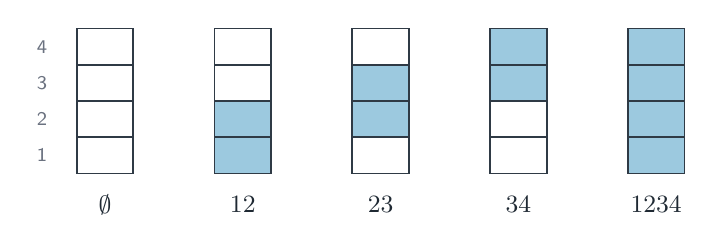
\begin{tikzpicture}[
  x=1cm,
  y=1cm,
  cell/.style={draw=stateStroke, line width=0.65pt},
  open/.style={cell, fill=white},
  filled/.style={cell, fill=stateFill},
  stateLabel/.style={font=\small\sffamily, text=stateText},
  rowLabel/.style={font=\scriptsize\sffamily, text=stateMuted, anchor=east}
]
  \def\cw{0.72}
  \def\ch{0.46}

  \foreach \row/\y in {4/1.38,3/0.92,2/0.46,1/0} {
    \node[rowLabel] at (-0.25,\y+0.23) {\row};
  }

  \begin{scope}[shift={(0,0)}]
    \path[open] (0,1.38) rectangle ++(\cw,\ch);
    \path[open] (0,0.92) rectangle ++(\cw,\ch);
    \path[open] (0,0.46) rectangle ++(\cw,\ch);
    \path[open] (0,0) rectangle ++(\cw,\ch);
    \node[stateLabel] at (0.36,-0.4) {$\emptyset$};
  \end{scope}

  \begin{scope}[shift={(1.75,0)}]
    \path[open] (0,1.38) rectangle ++(\cw,\ch);
    \path[open] (0,0.92) rectangle ++(\cw,\ch);
    \path[filled] (0,0.46) rectangle ++(\cw,\ch);
    \path[filled] (0,0) rectangle ++(\cw,\ch);
    \node[stateLabel] at (0.36,-0.4) {$12$};
  \end{scope}

  \begin{scope}[shift={(3.5,0)}]
    \path[open] (0,1.38) rectangle ++(\cw,\ch);
    \path[filled] (0,0.92) rectangle ++(\cw,\ch);
    \path[filled] (0,0.46) rectangle ++(\cw,\ch);
    \path[open] (0,0) rectangle ++(\cw,\ch);
    \node[stateLabel] at (0.36,-0.4) {$23$};
  \end{scope}

  \begin{scope}[shift={(5.25,0)}]
    \path[filled] (0,1.38) rectangle ++(\cw,\ch);
    \path[filled] (0,0.92) rectangle ++(\cw,\ch);
    \path[open] (0,0.46) rectangle ++(\cw,\ch);
    \path[open] (0,0) rectangle ++(\cw,\ch);
    \node[stateLabel] at (0.36,-0.4) {$34$};
  \end{scope}

  \begin{scope}[shift={(7,0)}]
    \path[filled] (0,1.38) rectangle ++(\cw,\ch);
    \path[filled] (0,0.92) rectangle ++(\cw,\ch);
    \path[filled] (0,0.46) rectangle ++(\cw,\ch);
    \path[filled] (0,0) rectangle ++(\cw,\ch);
    \node[stateLabel] at (0.36,-0.4) {$1234$};
  \end{scope}
\end{tikzpicture}
\end{document}
